%to have line numbers
%\RequirePackage{lineno}
\documentclass[10pt, letterpaper]{article}      
\usepackage[margin=.1cm,font=small,labelfont=bf]{caption}[2007/03/09]
%\usepackage{endnotes}
%\let\footnote=\endnote
\usepackage{setspace}
\usepackage{longtable}                        
\usepackage{anysize}                          
\usepackage{natbib}                           
%\bibpunct{(}{)}{,}{a}{,}{,}                   
\bibpunct{(}{)}{,}{a}{}{,}                   
\usepackage{amsmath}
\usepackage[% draft,
pdftex]{graphicx} %draft is a way to exclude figures                
\usepackage{epstopdf}
\usepackage{hyperref}                             % For creating hyperlinks in cross references
\hypersetup{pdfborder={0 0 0.4}} %have nice light boxes on refs

% \usepackage[margins]{trackchanges}

% \note[editor]{The note}
% \annote[editor]{Text to annotate}{The note}
%    \add[editor]{Text to add}
% \remove[editor]{Text to remove}
% \change[editor]{Text to remove}{Text to add}

%TODO make it more standard before submission: \marginsize{2cm}{2cm}{1cm}{1cm}
\marginsize{1cm}{1cm}{.5cm}{.5cm}%{left}{right}{top}{bottom}   
					          % Helps LaTeX put figures where YOU want
 \renewcommand{\topfraction}{1}	                  % 90% of page top can be a float
 \renewcommand{\bottomfraction}{1}	          % 90% of page bottom can be a float
 \renewcommand{\textfraction}{0.0}	          % only 10% of page must to be text

 \usepackage{float}                               %latex will not complain to include float after float

\usepackage[table]{xcolor}                        %for table shading
\definecolor{gray90}{gray}{0.90}
\definecolor{orange}{RGB}{255,128,0}

\renewcommand\arraystretch{.9}                    %for spacing of arrays like tabular

%-------------------- my commands -----------------------------------------
\newenvironment{ig}[1]{
\begin{center}
 %\includegraphics[height=5.0in]{#1} 
 \includegraphics[height=3.3in]{#1} 
\end{center}}

 \newcommand{\cc}[1]{
\hspace{-.13in}$\bullet$\marginpar{\begin{spacing}{.6}\begin{footnotesize}\color{blue}{#1}\end{footnotesize}\end{spacing}}
\hspace{-.13in} }

%-------------------- END my commands -----------------------------------------



%-------------------- extra options -----------------------------------------

%%%%%%%%%%%%%
% footnotes %
%%%%%%%%%%%%%

%\long\def\symbolfootnote[#1]#2{\begingroup% %these can be used to make footnote  nonnumeric asterick, dagger etc
%\def\thefootnote{\fnsymbol{footnote}}\footnote[#1]{#2}\endgroup}	%see: http://help-csli.stanford.edu/tex/latex-footnotes.shtml

%%%%%%%%%%%
% spacing %
%%%%%%%%%%%

% \abovecaptionskip: space above caption
% \belowcaptionskip: space below caption
%\oddsidemargin 0cm
%\evensidemargin 0cm

%%%%%%%%%
% style %
%%%%%%%%%

%\pagestyle{myheadings}         % Option to put page headers
                               % Needed \documentclass[a4paper,twoside]{article}
%\markboth{{\small\it Politics and Life Satisfaction }}
%{{\small\it Adam Okulicz-Kozaryn} }

%\headsep 1.5cm
% \pagestyle{empty}			% no page numbers
% \parindent  15.mm			% indent paragraph by this much
% \parskip     2.mm			% space between paragraphs
% \mathindent 20.mm			% indent math equations by this much

%%%%%%%%%%%%%%%%%%
% extra packages %
%%%%%%%%%%%%%%%%%%

\usepackage{datetime}


\usepackage[latin1]{inputenc}
\usepackage{tikz}
\usetikzlibrary{shapes,arrows,backgrounds}


%\usepackage{color}					% For creating coloured text and background
%\usepackage{float}
\usepackage{subfig}                                     % for combined figures

\renewcommand{\ss}[1]{{\colorbox{blue}{\bf \color{white}{#1}}}}
\newcommand{\ee}[1]{\endnote{\vspace{-.10in}\begin{spacing}{1.0}{\normalsize #1}\end{spacing}\vspace{.20in}}}
\newcommand{\emd}[1]{\ExecuteMetaData[/tmp/tex]{#1}} % grab numbers  from stata

%TODO before submitting comment this out to get 'regular fornt'
\usepackage{sectsty}
\allsectionsfont{\normalfont\sffamily}
\usepackage{sectsty}
\allsectionsfont{\normalfont\sffamily}
\renewcommand\familydefault{\sfdefault}

%\usepackage[margins]{trackchanges}
\usepackage{rotating}
\usepackage{catchfilebetweentags}

\usepackage{abstract}
\renewcommand{\abstractname}{}    % clear the title
\renewcommand{\absnamepos}{empty} % originally center
%-------------------- END extra options -----------------------------------------
\date{{}\today \hspace{.2in}\xxivtime}
\title{  % remember to have Vistula University!!
  Hey! Cities! Leave them kids alone!
}
\author{
% Adam Okulicz-Kozaryn\thanks{EMAIL: adam.okulicz.kozaryn@gmail.com
%   \hfill I thank XXX.  All mistakes are mine.} \\
% {\small Rutgers - Camden  % and Vistula University
% }
}

\begin{document}

%%\setpagewiselinenumbers
%\modulolinenumbers[1]
%\linenumbers

\bibliographystyle{/home/aok/papers/root/tex/ecta}
\maketitle
\vspace{-.4in}
\begin{center}

\end{center}


\begin{abstract}
\noindent strong effects! on the whole, 0.5 on 1-10 scale, and for some countries close to 1!
\end{abstract}
\vspace{.15in} 
\noindent{\sc %XXX TODO add to ebib as keyword PAPER-CODE-NAME and tag with ebib keywords 
}
\vspace{.25in} 

\begin{spacing}{1.4} %TODO MAYBE before submission can make it like 2.0
\rowcolors{1}{white}{gray90}

%  instead \ExecuteMetaData[../out/tex]{ginipov} do \emd{ginipov}

% \begin{figure}[H]
%  \includegraphics[height=3in]{../out/gov_res_trust.pdf}\centering\label{gov_res_trust}
% \caption{woo}
% \end{figure}


%TODO !!!! have input here aok_var_des

We know that adults tend to be less happy in cities across the world (except in
the poorest nations such as Sub-Saharan Africa) \citep{aok21}. But we do not
know about the children. 

\section{Happiness in Kids}

TODO: write sth about happness in kids; btw looks like they used normal happiness question; not smileys


\section{Data}

We use 2018 pisa from \url{https://www.oecd.org/pisa/data/2018database/}. Age is 15 to 16.3, so not kids kids but more like
little adolescents.

Urbanicity is recorded in  School questionnaire administered to school
principals:

Which of the following definitions best describes the community in which your school is located?
\begin{itemize}
\item A village, hamlet or ruralarea (fewer than 3 000 people)
\item A small town (3 000 to about 15 000 people)
\item A town (15 000 to about 100 000 people)
\item A city (100000 to about 1 000 000 people)
\item A large city (with over 1 000 000 people)
\end{itemize}

A nice feature of PISA data is that there are large cities, lt1m, in wvs for
instacne the top bin is only 500k. And it is missing for only 6 percent of
observations. 

a limitation is that we do not see a good health variable--exisiting ones are
missing for vast majroity. Health is of course a key happiness predictor, but
arguably less imoportant for kids as they are healthier than adults. 


PISA 2018 defines meaning in life as the extent to which 15-year-olds
comprehend, make sense of, or find significance in their lives
\citep{pisa18}. PISA 2018 asked students whether they agree or disagree (
"strongly disagree", "disagree", "agree", "strongly agree") with the following
statements: "My life has clear meaning or purpose"; "I have discovered a
satisfactory meaning in life"; and "I have a clear sense of what gives meaning
to my life". These statements were combined to create the index of meaning in
life



TODO varDes

\section{Results}

%meh have plenty of tables
% \begin{figure}[H]
%  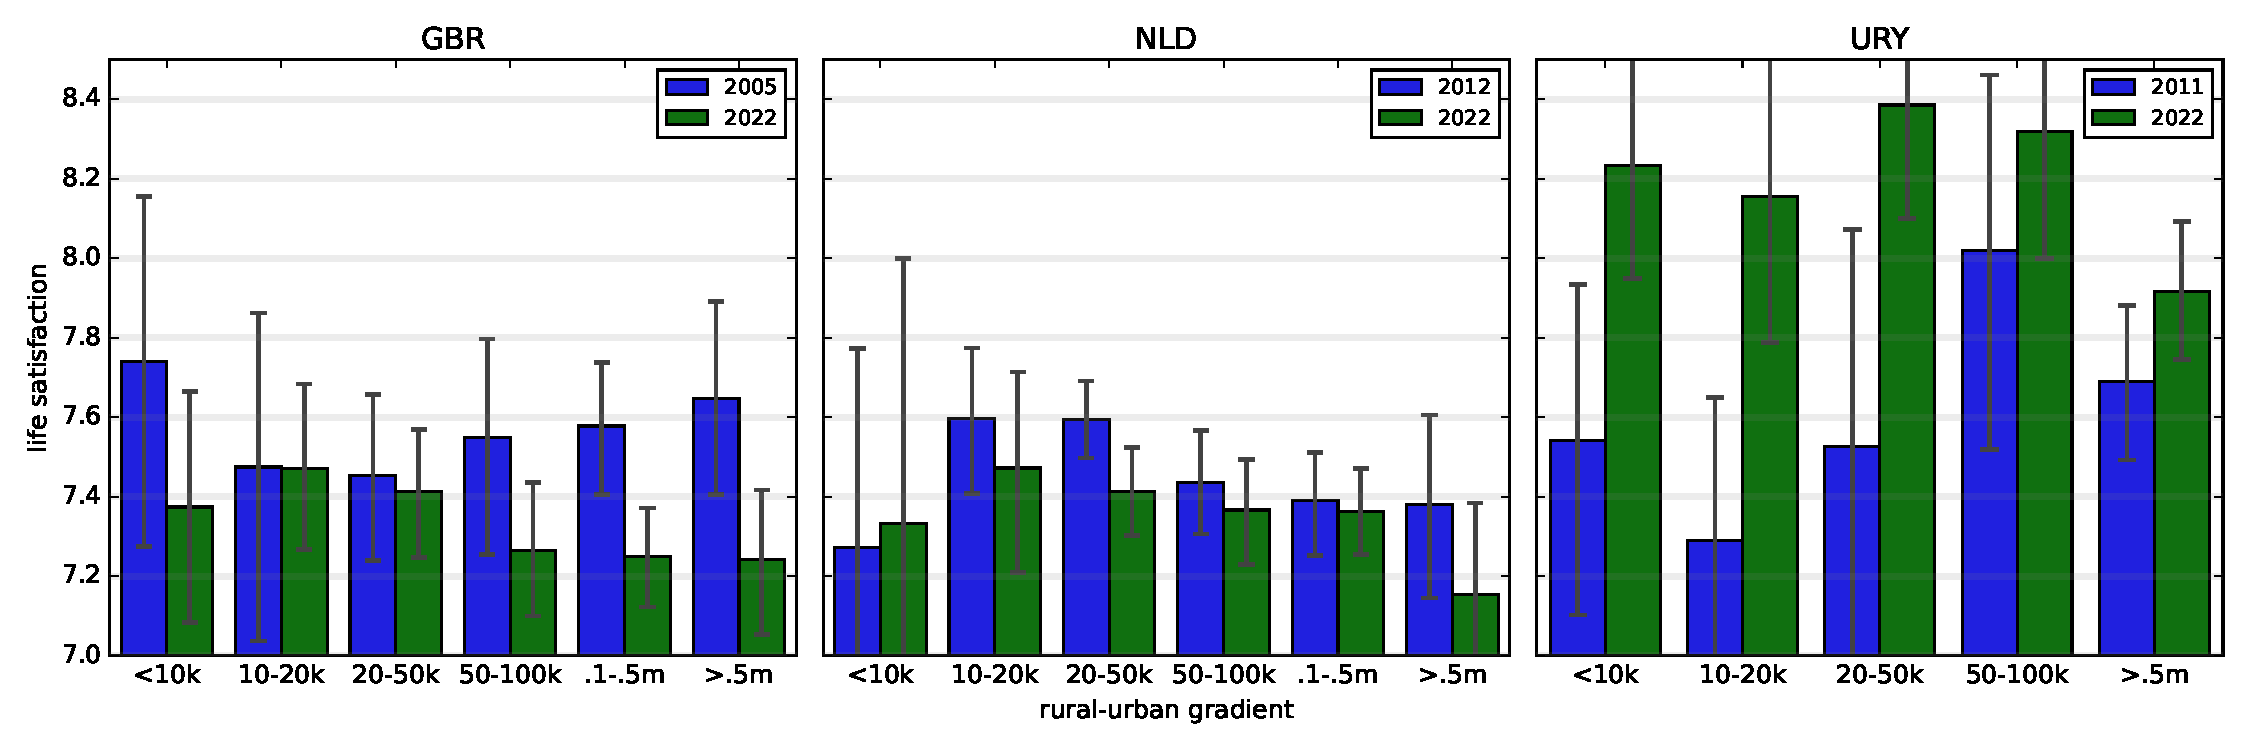
\includegraphics[height=3in]{bar.pdf}\centering\label{bar}
% \caption{Mean of life satisfaction and eudamonia by urbanicity.}
% \end{figure}


The differences are large--about .5 on 0-10 SWB scale. It needs to be remembered
that ecological variables have small effects on SWB as
 expected--most SWB is explained by genes \citep{schnittker08} and person level
 predictors \citep{veenhoven14b}). % . Still, the leading social scientists
 % such as Amartya Sen and Ed Diener advocate use of SWB for
 % public policy \citep{stiglitz09al,diener09}.
 %
 %
 %
 %
 And in a1-a3\footnote{Not
in a4 controling for country dummies.} there is a big
difference between the largest cities (gt1m) and everything else just as for
adults \citep{aok-ls_fisher16}. But interestingly, not necessarily like adults,
there is also a large gap between lt3k and 3-15k, again especially in models
a1-a3, perhaps in the open country there are best outdoor play opportunities for
the kids.

As in adults \citep{aok21}, addition of income/wealth makes results
stronger--income/wealth confounds with urbanicity.

In full model a4 results are strong, beta (fully standardized; not shown) for
gt1m is 65 percent of wealth.

Finally we split by gender in a4m and a4f--interestingly city penaly higher for female; arguably because fem more affected by urban crime 

\begin{table}[H]\centering\caption{OLS regressions of life satisfaction.} \label{regA} \begin{scriptsize} \begin{tabular}{p{2.2in}p{.6in}p{.6in}p{.6in}p{.6in}|p{.6in}p{.6in}p{.6in}p{.6in}p{.6in}p{.6 in}p{.6in}p{.6 in}}\hline                     &   $<.5m$   &     $>.5m$   &   $<.5m$   &     $>.5m$   &   URYrurTow   &     URYcity   \\
2022                &       -0.21** &       -0.41** &       -0.12** &       -0.23   &        0.75***&        0.23+  \\
constant            &        7.54***&        7.65***&        7.50***&        7.38***&        7.54***&        7.69***\\
N                   &        3111   &         521   &        3572   &         373   &        1154   &         836   \\
 \hline\multicolumn{4}{l}{*p$<$0.05 **p$<$0.01 ***p$<$0.001} \end{tabular}\end{scriptsize}\end{table}




\begin{spacing}{.9} \begin{table}[H]\centering   \begin{scriptsize} \begin{tabular}{p{.5in}p{.5in}p{.5in}p{.5in}p{.5in}p{.5in}p{.5in}p{.5in}p{.5in}p{.5in}p{.5
                                                                      in}p{.5in}p{.5
                                                                      in}}\hline
                                                                      \input{../out/a4cou.tex}
                                                                      \hline *
                                                                      p$<$0.05,
                                                                      $+$
                                                                      p$<$0.1;
                                                                      robust std
                                                                      err \end{tabular}\end{scriptsize}\caption{\label{a4cou}OLS
                                                                    regressions
                                                                    of life satisfaction on
                                                                    place size
                                                                    for each
                                                                    country
                                                                    separately
                                                                    includiOBng
                                                                    covariates
                                                                    from a4 (not
                                                                    shown). Only
                                                                  LBN and HUN
                                                                  marginally
                                                                  happier in
                                                                  cities lt1m
                                                           }\end{table} \end{spacing}


\subsection{Eudamonia}

in table \ref{regB} different from lifests, biggest hit from lt3k to 3-15k in b1-b3, and in b4
controllig for countruy dummies rather smooth gradient. females aboy 2x less
eudamonia than males in urb v rural

\begin{table}[H]\centering\caption{OLS regressions of Eudamonia.} \label{regB} \begin{scriptsize} \begin{tabular}{p{2.2in}p{.6in}p{.6in}p{.6in}p{.6in}|p{.6in}p{.6in}p{.6in}p{.6in}p{.6in}p{.6 in}p{.6in}p{.6 in}}\hline                     &   $<.5m$   &     $>.5m$   &   $<.5m$   &     $>.5m$   &   URYrurTow   &     URYcity   \\
2022                &       -0.18*  &       -0.39+  &       -0.20***&       -0.45** &        0.42***&        0.21   \\
income              &        0.09***&        0.01   &        0.06***&        0.14***&        0.07*  &        0.13***\\
age                 &       -0.03*  &       -0.08** &       -0.02+  &       -0.06+  &        0.00   &       -0.06** \\
age2                &        0.00** &        0.00** &        0.00** &        0.00*  &       -0.00   &        0.00** \\
male                &       -0.18** &       -0.13   &       -0.11*  &       -0.27+  &        0.06   &        0.19   \\
married or living together as married&        0.53***&        0.74***&        0.44***&        0.23   &        0.46** &        0.06   \\
divorced/separated/widowed&        0.07   &        0.15   &       -0.11   &       -0.14   &       -0.37+  &       -0.19   \\
autonomy            &       -0.11*  &       -0.07   &       -0.11** &       -0.01   &       -0.06   &        0.06   \\
freedom             &        0.44***&        0.42***&        0.35***&        0.43***&        0.43***&        0.36***\\
trust               &        0.12+  &        0.42** &        0.43***&        0.28+  &       -0.05   &        0.10   \\
postmaterialist     &       -0.05   &       -0.18   &       -0.11*  &        0.14   &       -0.02   &        0.15   \\
god important       &        0.01   &        0.05*  &        0.02*  &       -0.01   &        0.05** &        0.06** \\
constant            &        4.08***&        5.95***&        4.59***&        4.80***&        3.47***&        4.58***\\
N                   &        1985   &         309   &        2283   &         237   &         736   &         579   \\
 \hline\multicolumn{4}{l}{*p$<$0.05 **p$<$0.01 ***p$<$0.001} \end{tabular}\end{scriptsize}\end{table}

in atble \ref{b4cou} urban eudamia penalty is less clear than life
satisfaction--while most countries do have urban penalty, there is a handful
with urban eudamonic premium


\begin{spacing}{.9} \begin{table}[H]\centering   \begin{scriptsize} \begin{tabular}{p{.5in}p{.5in}p{.5in}p{.5in}p{.5in}p{.5in}p{.5in}p{.5in}p{.5in}p{.5in}p{.5
                                                                      in}p{.5in}p{.5
                                                                      in}}\hline
                                                                      \input{../out/b4cou.tex}
                                                                      \hline *
                                                                      p$<$0.05,
                                                                      $+$
                                                                      p$<$0.1;
                                                                      robust std
                                                                      err \end{tabular}\end{scriptsize}\caption{\label{b4cou}OLS
                                                                    regressions
                                                                    of Eudamonia on
                                                                    place size
                                                                    for each
                                                                    country
                                                                    separately
                                                                    including
                                                                    covariates
                                                                    from b4 (not
                                                                    shown). Most
                                                                    countries
                                                                    eudamoinc
                                                                    urban
                                                                    penalty, but
                                                                    a
                                                                    handful of
                                                                    countries
                                                                    have premium
                                                           }\end{table} \end{spacing}




\section{Conclusion and discussion}

Future research:
Arguably after the pandemic cities became even more unhappy just as adults did
\textbf{??blind for peer-review}

                                                       
% %table centered on decimal points:)
% \begin{table}[H]\centering\footnotesize
% \caption{\label{freq_im_god} importance of God}
% \begin{tabular} {@{} lrrrr @{}}   \hline 
% Item& Number & Per cent   \\ \hline
% 1(not at all)&    9,285&  9\\
% 2&    3,555&        3\\
% 3&    3,937&        4\\
% 4&    2,888&        3\\
% 5&    7,519&        7\\
% 6&    5,175&        5\\
% 7&    6,050&        6\\
% 8&    8,067&        8\\
% 9&    8,463&        8\\
% 10&   52,385&       49\\
% Total&  107,324&      100\\ \hline
% \end{tabular}\end{table}


% % Define block styles
% \tikzstyle{block} = [rectangle, draw, fill=black!20, 
%     text width=10em, text centered, rounded corners, minimum height=4em]
% \tikzstyle{b} = [rectangle, draw,  
%     text width=6em, text centered, rounded corners, minimum height=4em]
% \tikzstyle{line} = [draw, -latex']
% \tikzstyle{cloud} = [draw, ellipse,fill=black!20, node distance = 5cm,
%     minimum height=2em]
    
% \begin{tikzpicture}[node distance = 2cm, auto]
%     % Place nodes
%     \node [block] (lib) {liberalism, egalitarianism, welfare};
%     \node [block, below of=lib] (con) {conservatism, competition, individualism};
%     \node [cloud, right of=con] (ls) {well-being};
%     \node [block, below of=ls] (cul) {genes, culture};
%     \node [b, left of =lib, node distance = 4cm] (c) {country-level};
%     \node [b, left of =con,  node distance = 4cm] (c) {person-level};
%     % Draw edges
%     \path [line] (lib) -- (ls);
%     \path [line] (con) -- (ls);
%     \path [line,dashed] (cul) -- (ls);
% \end{tikzpicture}


%PUT THIS NOTE, polish and put to /root/author_what_data --ALWAYS
%stick here stuff as i run it!!! maybe comment out later...


TODO: have separate som-r.tex as opposed to having it below; and in paper say
see supplemetary material as opposed to see appendix!

 \section*{\Huge ONLINE APPENDIX}
 \textbf{[note: this section will NOT be a part of the final version of
   the manuscript, but will be available online instead]} %hence everything below
                                 %is organized byu section, not subsection
% !!!
% have most of the stuff outputted to online appendix:)--start with that and then
% select stuff to paper--have brief narrative describng patterns in online app too
% !!!

% \section*{Variables' definitions, coding, and distributions}
% \label{app_var_des}



\begin{spacing}{.9} \begin{table}[H]\centering   \begin{scriptsize} \begin{tabular}{p{.5in}p{.5in}p{.5in}p{.5in}p{.5in}p{.5in}p{.5in}p{.5in}p{.5in}p{.5in}p{.5
                                                                      in}p{.5in}p{.5
                                                                      in}}\hline
                                                                      \input{../out/a1.tex}
                                                                      \hline *
                                                                      p$<$0.05,
                                                                      $+$
                                                                      p$<$0.1;
                                                                      robust std
                                                                      err \end{tabular}\end{scriptsize}\caption{\label{d1}OLS
                                                                    regressions
                                                                    of SWB on
                                                                    place size
                                                                    only
                                                                    (bivariate; a1)
                                                                    for each
                                                                    country
                                                                    separately. barely
                                                                    anything
                                                                    like france
                                                                    and 2 more
                                                                  }\end{table} \end{spacing}

 
% %\input{/tmp/a.tex} %aok_var_des

% % \begin{spacing}{.9}
% %   \begin{table}[H]\centering \caption{Summary statistics.} \label{sumSta} \begin{scriptsize} \begin{tabular}{p{1.8in}p{.5in}p{.5in}p{.5in}p{.5in}p{.5in}p{.5in}p{.5in}p{.5in}p{.5in}p{.5
% %             in}p{.5in}p{.5 in}}\hline
% %         \input{/tmp/aha2.tex}
% %          \end{tabular}\end{scriptsize}\end{table}
% % \end{spacing}

% % \begin{spacing}{.9}
% %   \begin{table}[H]\centering \caption{Correlation matrix.} \label{sumSta} \begin{scriptsize} \begin{tabular}{@{}
% %           p{1.2in} rrrrrrrrrrrrr @{}}\hline
% %         \input{/tmp/ahb2.tex}\hline
% %          \end{tabular}\end{scriptsize}\end{table}
% % \end{spacing}



% Table XXX shows variable distributions. If a variable has more than
% 10 categories it is classified into bins...

% %\input .... %TODO !!!! have input here histograms

% \section*{Additional Descriptive Statistics}
% \label{app_des_sta}

% %make sure i have [H] or h! ???
% % \begin{table}[H]
% % \caption{}
% % \centering
% % \label{}
% % \begin{scriptsize}
% % \input{../out/reg_c.tex}
% % \end{scriptsize}
% % \end{table}

%\newpage
%\theendnotes
\bibliography{/home/aok/papers/root/tex/ebib.bib,pisa.bib}

\end{spacing}
\end{document}
